\chapter{Neural Networks}
In this chapter, we discuss \href{https://en.wikipedia.org/wiki/Artificial_neural_network}{artificial neural networks}.
Many of the most visible breakthroughs in artificial intelligence have been achieved through the use of neural
networks: 
\begin{enumerate}
\item The current system used by Google to \href{https://translate.google.com}{automatically translate} web
      pages is called 
      ``\href{https://en.wikipedia.org/wiki/Google_Neural_Machine_Translation}{Google Neural Machine Translation}''
      and, as the name suggests, is based on neural networks. 
\item \href{https://www.deepl.com/translator}{DeepL} is another translator that is based on neural networks.      
\item \href{https://en.wikipedia.org/wiki/AlphaGo}{AlphaGo} uses neural networks together with tree search
      \cite{silver:2016}.  It has \href{https://en.wikipedia.org/wiki/AlphaGo_versus_Ke_Jie}{beaten} 
      the world champion \href{https://en.wikipedia.org/wiki/Ke_Jie}{Ke Jie} in the game of
      \href{https://en.wikipedia.org/wiki/Go_(game)}{Go}. AlphaGo has been succeeded by
      \href{https://en.wikipedia.org/wiki/AlphaZero}{AlphaZero}, which is even stronger than AlphaGo.
\item \blue{Image recognition} is best done via neural networks.
\item \href{https://en.wikipedia.org/wiki/Autonomous_car}{Autonomous driving} makes heavy use of neural networks.
\end{enumerate}
The list given above is far from being complete.  In this chapter, we will only discuss 
\href{https://en.wikipedia.org/wiki/Feedforward_neural_network}{feedforward neural networks}.  Although recently both 
\href{https://en.wikipedia.org/wiki/Convolutional_neural_network}{convolutional neural networks} and
\href{https://en.wikipedia.org/wiki/Recurrent_neural_network}{recurrent neural networks} have gotten a lot of
attention, these type of neural networks are more difficult to understand and are therefore beyond the scope of this
introduction.  The rest of this chapter is strongly influenced by the online book 
\\[0.2cm]
\hspace*{1.3cm}
\href{http://neuralnetworksanddeeplearning.com/index.html}{http://neuralnetworksanddeeplearning.com/index.html}
\\[0.2cm]
that has been written by Michael Nielsen \cite{nielsen:2015}.  This book is easy to read, carefully written, and
free to access.  I recommend this book to anybody who wants to dive deeper into the fascinating topic of neural
networks.

We proceed to give an overview of the content of this chapter.
\begin{enumerate}
\item We start with the definition of \blue{feed forward} neural networks and discuss their \blue{topology}.
\item We introduce \blue{forward propagation}, which is the way a neural network computes its predictions.
\item Similarly to our treatment of logistic regression, we define a cost function that measure the quality of
      the predictions of a neural network on a training set.  In order to minimize this cost function using
      gradient descent, we have to compute the \blue{gradient} of the cost function with respect to the weights of the
      neural network.  The algorithm which is used to compute this gradient is called \blue{backpropagation}.
\item In order to find the minimum of the cost function efficiently, we need an improved version of
      \blue{gradient descent}.  This improved version is known as \blue{stochastic gradient descent}.
\item After having covered the theory, we implement a simple neural network that is able to recognize
      \blue{handwritten digits}.
\item Finally, we discuss \href{https://www.tensorflow.org}{TensorFlow}, which is an open source software
      library for machine learning in general and neural networks in particular.
\end{enumerate}

\section{Feedforward Neural Networks}
A neural network is built from \blue{neurons}.  Neural networks are inspired by biological 
\href{https://en.wikipedia.org/wiki/Neuron}{neurons}.  However, in order to understand artificial neural
networks it is not necessary to know how biological neurons work and it is definitely not necessary to
understand how networks of biological neurons, i.e.~brains, work\footnote{
  Actually, when it comes to brains, although there are many speculations, surprisingly little is known for a fact.  
}.  
Instead, we will use a mathematical abstraction of neurons that will serve as the foundation of the theory
developed in this chapter.  At the abstraction level that we are using to look at neural networks, a single neuron
with $m$ inputs is specified by a pair $\langle \mathbf{w}, b\rangle$ where the vector $\mathbf{w} \in \mathbb{R}^m$ is called the \blue{weight vector} and 
the number $b \in \mathbb{R}$ is called the \blue{bias}.   
Conceptually, a neuron is a function that maps an input vector $\mathbf{x} \in \mathbb{R}^m$ into the set
$\mathbb{R}$ of the real numbers.  This function is defined as follows: 
\\[0.2cm]
\hspace*{1.3cm}
$\ds \mathbf{x} \mapsto a(\mathbf{x} \cdot \mathbf{w} + b)$.
\\[0.2cm]
Here, $a$ is called the \blue{activation function}.  \index{activation function} In our applications, we will
use the sigmoid function as our activation function.  This function has been defined previously in Definition
\ref{def:sigmoid} on page \pageref{def:sigmoid} as follows:
\\[0.2cm]
\hspace*{1.3cm}
$\ds a(t) := S(t) = \frac{1}{1 + \exp(-t)}$.
\\[0.2cm]
Another useful activation function is the so called
\href{https://en.wikipedia.org/wiki/Rectifier_(neural_networks)}{ReLU function}, \index{ReLU function}
which is defined as 
\\[0.2cm]
\hspace*{1.3cm}
$a(t) = \max(0, x)$.
\\[0.2cm]
The abbreviation ReLU is short for \blue{rectified linear unit}. \index{rectified linear unit}
The function modelling the neuron can be written more explicitly using index notation.  If
\\[0.2cm]
\hspace*{1.3cm}
$\mathbf{w} = \langle w_1, \cdots, w_m \rangle^\top$ 
\\[0.2cm]
is the weight vector and 
\\[0.2cm]
\hspace*{1.3cm}
$\mathbf{x} = \langle x_1, \cdots, x_m \rangle^\top$
\\[0.2cm]
is the input vector, and $b\in \mathbb{R}$ is the \blue{bias}, \index{bias} then we have
\\[0.2cm]
\hspace*{1.3cm}
$\ds \mathbf{x} \mapsto S\left(\biggl(\sum\limits_{i=1}^m x_i \cdot w_i\biggr) + b\right)$.
\\[0.2cm]
If we compare this function to a similar function appearing in the last chapter, you will notice 
that a single neuron works just like a classifier in logistic regression.  The only difference is that the bias $b$
is now explicit in our notation.  In logistic regression, we had assumed that the first component $x_1$ of our
feature vector $\mathbf{x}$ was always equal to $1$.  This assumption enabled us to incorporate the bias $b$ into the
weight vector $\mathbf{w}$.

\begin{figure}[!h]
  \centering
  \vspace*{-2cm}
  \epsfig{file=Figures/nn1.pdf,scale=1.5}
    \vspace*{-2cm}
   \caption{A neural network with topology $[3, 6, 4, 2]$.}
  \label{fig:nn1.pdf}
\end{figure}

A \blue{feedforward neural network} \index{feed forward neural network} is a layered network of neurons.
Formally, the \blue{topology} \index{topology} of a neural network is 
given by a number $L \in \mathbb{N}$ and a list $[m(1), \cdots, m(L)]$ of $L$ natural numbers.  The number
$L$ is called the \blue{number of layers} \index{number of layers} and for $l \in \{2,\cdots,L\}$ the number $m(l)$ is the number of
neurons in the $l$-th layer.  The first layer is called the \blue{input layer}. \index{input layer}
The input layer does not contain neurons but instead just contains \blue{input nodes}. \index{input node} The
last layer (i.e.~the layer with index $L$) is called the \blue{output layer} \index{output layer} and the
remaining layers are called \blue{hidden layers}.  \index{hidden layer} If there is more than one hidden layer,
the neural network is called a \blue{deep neural network}. \index{deep neural network} Figure \ref{fig:nn1.pdf}
on page \pageref{fig:nn1.pdf} shows a small neural network with two hidden layers.  Including the input layer
it has four layers and its topology is given by the list $[3, 6, 4, 2]$.  A larger neural network with three
hidden layers is shown in Figure \ref{fig:nn2.pdf} on page \pageref{fig:nn2.pdf}.  I have written a small
Jupyter notebook that can be used to draw diagrams of this kind. This notebook is available at
\href{https://github.com/karlstroetmann/Artificial-Intelligence/blob/master/Python/7%20Neural%20Networks/NN-Architecture.ipynb}{NN-Architecture.ipynb}
in the \texttt{Python} subdirectory of my GitHub repository for this lecture. 


\begin{figure}[!h]
  \centering
  \vspace*{-2cm}
  \epsfig{file=Figures/nn2.pdf,scale=1.5}
  \vspace*{-2cm}
   \caption{A neural network with topology $[8, 12, 8, 6, 3]$.}
  \label{fig:nn2.pdf}
\end{figure}


If the topology of a neural network is  $[m(1), \cdots, m(L)]$, the \blue{input dimension} \index{input dimension}
is defined as $m(1)$.  Similarly, the \blue{output dimension} \index{output dimension} is defined as $m(L)$.
The feedforward neural networks discussed in this chapter are \blue{fully connected}:  \index{fully connected}
Every node in the $l$-th layer is connected to every node in the $(l+1)$-th layer via a \blue{weight}.
\index{weight of NN}
The weight $w_{j,k}^{(l)}$ is the weight of the connection from the $k$-th neuron in layer $l-1$ to
the $j$-th neuron in layer $l$.  The weights in layer $l$ are combined into the \blue{weight matrix} $W^{(l)}$
\index{weight matrix} of the layer $l$: This matrix is defined as
\\[0.2cm]
\hspace*{1.3cm}
$\ds W^{(l)} := \bigl( w_{j,k}^{(l)} \bigr)$.
\\[0.2cm]
Note that $W^{(l)}$ is an $m(l) \times m(l-1)$ matrix, i.e.~we have
\\[0.2cm]
\hspace*{1.3cm}
$\ds W^{(l)} \in \mathbb{R}^{m(l) \times m(l-1)}$.
\\[0.2cm]
The $j$-th neuron in layer $l$ has the \blue{bias} $b_j^{(l)}$.  These biases of layer $l$ are combined into
the \blue{bias vector} \index{bias vector}
\\[0.2cm]
\hspace*{1.3cm}
$\mathbf{b}^{(l)} := \bigl\langle b_1^{(l)}, \cdots, b_{m(l)}^{(l)} \bigr\rangle^\top$.
\FloatBarrier

\noindent
The \blue{activation} of the $j$-th neuron
in layer $l$ is denoted as $a_j^{(l)}$ and is defined recursively as follows:
\begin{enumerate}
\item For the input layer we have
      \begin{equation}
        \label{eq:FF1}
       a^{(1)}_j(\mathbf{x}) := x_j.
       \tag{FF1}
      \end{equation}
      To put it differently, the input vector $\mathbf{x}$ is the activation of the input nodes.
\item For all other layers we have
      \begin{equation}
         \label{eq:FF2}
         a_j^{(l)}(\mathbf{x}) := 
             S\left(\Biggl(\sum\limits_{k=1}^{m(l-1)} w_{j,k}^{(l)}\cdot a_k^{(l-1)}(\mathbf{x})\Biggr) + b_{j}^{(l)}\right) 
        \quad \mbox{for all $l \in \{2, \cdots, L\}$}.
       \tag{FF2}
\end{equation}
\end{enumerate}
The \blue{activation vector} \index{activation vector} of layer $l$ is defined as
\\[0.2cm]
\hspace*{1.3cm}
$\mathbf{a}^{(l)}(\mathbf{x}) := \bigl\langle a_1^{(l)}(\mathbf{x}), \cdots, a_{m(l)}^{(l)}(\mathbf{x}) \bigr\rangle^\top$.
\\[0.2cm]
Using vector notation, the \blue{feed forward equations} \index{feed forward equations}
(\ref{eq:FF1}) and (\ref{eq:FF2}) can be rewritten as follows:
\begin{align}
  \label{eq:FF1v}
  \mathbf{a}^{(1)}(\mathbf{x}) & := \mathbf{x},
  \tag{FF1v} \\ 
  \label{eq:FF2v}
  \mathbf{a}^{(l)}(\mathbf{x}) & := 
  S\Bigl( W^{(l)} \cdot \mathbf{a}^{(l-1)}(\mathbf{x}) + \mathbf{b}^{(l)}\Bigr)
  \quad \mbox{for all $l \in \{2, \cdots, L\}$}.
  \tag{FF2v}
\end{align}

The output of our neural network for an input $\mathbf{x}$ is given by the neurons in the output
layer,  i.e.~the output vector 
$\mathbf{o}(\mathbf{x}) \in \mathbb{R}^{m(L)}$ is defined as 
\\[0.2cm]
\hspace*{1.3cm}
$\mathbf{o}(\mathbf{x}) :=
 \bigl\langle a^{(L)}_1(\mathbf{x}), \cdots, a^{(L)}_{m(L)}(\mathbf{x}) \bigr\rangle^\top = \mathbf{a}^{(L)}(\mathbf{x})$.
\\[0.2cm]
Note that the equations (\ref{eq:FF1}) and (\ref{eq:FF2}) describe how information propagates
through the neural network: 
\begin{enumerate}
\item Initially, the input vector $\mathbf{x}$ is given and stored in the input layer of the neural network:
      \\[0.2cm]
      \hspace*{1.3cm}
      $\mathbf{a}^{(1)}(\mathbf{x}) := \mathbf{x}$.
\item The first layer of neurons, which is the second layer of nodes,  is activated and computes the activation
      vector $\mathbf{a}^{(2)}$ according to the formula
      \\[0.2cm]
      \hspace*{1.3cm}
      $\mathbf{a}^{(2)}(\mathbf{x}) := S\bigl(W^{(2)} \cdot \mathbf{a}^{(1)}(\mathbf{x}) + \mathbf{b}^{(2)}\bigr) = 
                                        S\bigl(W^{(2)} \cdot \mathbf{x} + \mathbf{b}^{(2)}\bigr)
      $.
\item The second layer of neurons, which is the third layer of nodes,  is activated and computes the activation
      vector $\mathbf{a}^{(3)}(\mathbf{x})$ according to the formula
      \\[0.2cm]
      \hspace*{1.3cm}
      $\mathbf{a}^{(3)}(\mathbf{x}) := S\bigl(W^{(3)} \cdot \mathbf{a}^{(2)}(\mathbf{x}) + \mathbf{b}^{(3)}\bigr)
                          = S\Bigl(W^{(3)} \cdot S\bigl(W^{(2)} \cdot \mathbf{x} + \mathbf{b}^{(2)}\bigr) + \mathbf{b}^{(3)}\Bigr)
        $
\item This proceeds until the output layer is reached and the output
      \\[0.2cm]
      \hspace*{1.3cm}
      $\mathbf{o}(\mathbf{x}) := \mathbf{a}^{(L)}(\mathbf{x})$
      \\[0.2cm]
      has been computed.  As long as we use the sigmoid function as our activation function, every neuron of
      the neural network performs logistic regression. 
\end{enumerate}
Next, we assume that we have $n$ \blue{training examples} 
\\[0.2cm]
\hspace*{1.3cm}
$\bigl\langle \mathbf{x}^{(i)}, \mathbf{y}^{(i)} \bigr\rangle$ \quad for $i=1,\cdots,n$ 
\\[0.2cm]
such that 
\\[0.2cm]
\hspace*{1.3cm}
$\mathbf{x}^{(i)} \in \mathbb{R}^{m(1)}$ and $\mathbf{y}^{(i)} \in \mathbb{R}^{m(L)}$.
\\[0.2cm]
Our goal is to choose the weight matrices $W^{(l)}$ and the bias vectors $\mathbf{b}^{(l)}$ in a way such that
\\[0.2cm]
\hspace*{1.3cm}
$\mathbf{o}\bigl(\mathbf{x}^{(i)}\bigr) = \mathbf{y}^{(i)}$ \quad for all $i \in \{1,\cdots,n\}$.
\\[0.2cm]
Unfortunately, in general we will not be able to achieve equality for all  $i \in \{1,\cdots,n\}$.
Therefore, our goal is to minimize the \blue{error} instead.  To be more precise, the 
\blue{quadratic error cost function} \index{quadratic error cost function} is defined as 
\\[0.2cm]
\hspace*{1.3cm}
$\ds C\Bigr(W^{(2)}, \cdots, W^{(L)}, \mathbf{b}^{(2)}, \cdots, \mathbf{b}^{(L)};
     \mathbf{x}^{(1)}, \mathbf{y}^{(1)}, \cdots, \mathbf{x}^{(n)},\mathbf{y}^{(n)} \Bigr) := 
 \frac{1}{2 \cdot n} \cdot \sum\limits_{i=1}^n \Bigl(\mathbf{o}\bigl(\mathbf{x}^{(i)}\bigr) - \mathbf{y}^{(i)}\Bigr)^2
$.
\\[0.2cm]
Note that this cost function is additive in the training examples $\bigl\langle \mathbf{x}^{(i)}, \mathbf{y}^{(i)} \bigr\rangle$.
In order to simplify the notation we define
\\[0.2cm]
\hspace*{1.3cm}
$\ds C_{\mathbf{x}, \mathbf{y}}\Bigr(W^{(2)}, \cdots, W^{(L)}, \mathbf{b}^{(2)}, \cdots, \mathbf{b}^{(L)}\Bigr) := 
 \frac{1}{2} \cdot \Bigl(\mathbf{a}^{(L)}\bigl(\mathbf{x}\bigr) - \mathbf{y}\Bigr)^2
$,
\\[0.2cm]
i.e.~$C_{\mathbf{x},\mathbf{y}}$ is the part of the cost function that is associated with a single training example $\pair(\mathbf{x},\mathbf{y})$.
Then we have
\\[0.2cm]
\hspace*{1.3cm}
$
\begin{array}{cl}
    & \ds C\Bigr(W^{(2)}, \cdots, W^{(L)}, \mathbf{b}^{(2)}, \cdots, \mathbf{b}^{(L)};
     \mathbf{x}^{(1)}, \mathbf{y}^{(1)}, \cdots, \mathbf{x}^{(n)},\mathbf{y}^{(n)} \Bigr) \\
:= & \ds \frac{1}{n} \cdot \sum\limits_{i=1}^n C_{\mathbf{x}^{(i)}, \mathbf{y}^{(i)}}\Bigr(W^{(2)}, \cdots W^{(L)}, \mathbf{b}^{(2)}, \cdots, \mathbf{b}^{(L)}\Bigr).
\end{array}
$
\\[0.2cm]
As the notation
\\[0.2cm]
\hspace*{1.3cm}
$C_{\mathbf{x}, \mathbf{y}}\Bigr(W^{(2)}, \cdots, W^{(L)}, \mathbf{b}^{(2)}, \cdots, \mathbf{b}^{(L)}\Bigr)$
\\[0.2cm]
is far too heavy, we will abbreviate this term as $C_{\mathbf{x}, \mathbf{y}}$ in the following
discussion of the backpropagation algorithm.  Similarly, we abbreviate the quadratic error cost function as $C$.
Our goal is to choose the weight matrices $W^{(l)}$ and the bias vectors $\mathbf{b}^{(l)}$ such that the
quadratic error cost function $C$ is minimized.  We will use a variation of
\href{https://ml-cheatsheet.readthedocs.io/en/latest/gradient_descent.html}{gradient descent} to
\index{gradient descent} find this minimum\footnote{
  In logistic regression we have tried to \emph{maximize} the log-likelihood.  Here, instead
  we \emph{minimize} the quadratic error cost function.  Hence, instead of gradient \emph{ascent} we use
  gradient \emph{descent}.  
}.
Unfortunately, the cost function $C$ when regarded as a function of the weights and biases has many local 
minima.  Hence, in practical applications all we can hope for is to find a local minimum that is good enough
for the goal that we want to achieve.


\section{Backpropagation}
There are three reasons for the recent success of neural networks.
\begin{enumerate}
\item The computing power that is available today has vastly increased in the last 20 years.
      For example, today the
      \href{https://www.nvidia.com/en-us/geforce/graphics-cards/30-series/rtx-3090/}{NVIDIA RTX 3090}
      graphic card offers 35 teraflops in single precision performance. It needs a power supply that
      outputs 750 watt. Contrast this with \href{https://en.wikipedia.org/wiki/ASCI_White}{ASCI White}, which
      was the most powerful supercomputer in 2000: According to the article
      ``\href{https://en.wikipedia.org/wiki/History_of_supercomputing}{History of Supercomputing}'', 
      it  offered a performance of 7.2 teraflops and needed 6 megawatt to operate.  The cost to build ASCI
      White was about $110,000,000\,\symbol{36}$.   To compare, the NVIDIA RTX 3090 costs $1,\!499\,\symbol{36}$.
\item The breakthrough in the theory of neural networks was the rediscovering of the
      \href{https://en.wikipedia.org/wiki/Backpropagation}{backpropagation algorithm} \index{backpropagation} by
      David Rumelhart, Geoffrey Hinton, and Ronald Williams \cite{rumelhart:1986} in 1986.  
      The backpropagation algorithm had first been discovered by Arthur E.~Bryson, Jr.~and Yu-Chi Ho
      \cite{bryson:1969}.  In recent years, there have been a number of other theoretical advances that have
      helped in speeding up the learning algorithms for neural networks.
\item Lastly, as neural networks have large sets of parameters, they need large sets of training examples.  The
      recent digitization of our society has made these large data sets available.
\end{enumerate}
Essentially, the \blue{backpropagation} algorithm is an efficient way to compute the partial derivatives of the
cost function $C$ with respect to the weights $w_{j,k}^{(l)}$ and the biases $b_j^{(l)}$.  Before we can
proceed to compute these partial derivatives, we need to define some auxiliary variables. 

\subsection{Definition of some Auxiliary Variables}
We start by defining the auxiliary variables $z_j^{(l)}$.
 The expressions $z_j^{(l)}$  are defined as the inputs of the activation function $S$ of the $j$-th neuron in
 layer $l$:
\\[0.2cm]
\hspace*{1.3cm}
$\ds z_j^{(l)} := \left(\sum\limits_{k=1}^{m(l-1)}  w_{j,k}^{(l)} \cdot a_k^{(l-1)}\right) + b_j^{(l)}$
\quad for all  $j \in \{1, \cdots, m(l)\}$ and $l \in \{2,\cdots,L\}$.
\\[0.2cm]
Of course, the term  $a_k^{(l-1)}$ really is a function of the input vector $\mathbf{x}$.  However, it is better to suppress
this dependence in the notation since otherwise the formulas get too cluttered.
Essentially, $z_j^{(l)}$ is the input to the sigmoid function when the activation $a_j^{(l)}$ is computed,
i.e.~we have
\\[0.2cm]
\hspace*{1.3cm}
$a_j^{(l)} = S\Bigl(z_j^{(l)}\Bigr)$.
\\[0.2cm]
Later, we will see that the partial derivatives of the cost function $C_{\mathbf{x}, \mathbf{y}}$ with respect to both the weights
$w_{j,k}^{(l)}$ and the biases $b_j^{(l)}$ can be computed easily if we first compute the partial derivatives
of $C_{\mathbf{x}, \mathbf{y}}$ with respect to $z_j^{(l)}$.  Therefore we define
\\[0.2cm]
\hspace*{1.3cm}
$\ds\varepsilon_j^{(l)} := \frac{\partial C_{\mathbf{x}, \mathbf{y}}}{\partial z_j^{(l)}}$ \quad for all $j \in \{1, \cdots, m(l)\}$ and $l \in \{2,\cdots, L\}$,
\\[0.2cm]
that is we regard $C_{\mathbf{x}, \mathbf{y}}$ as a function of the $z_j^{(l)}$ and take the partial
derivatives according to these variables.  
Note that $\varepsilon_j^{(l)}$ depends on both $\mathbf{x}$ and $\mathbf{y}$.  
We call  $\varepsilon_j^{(l)}$ the \blue{error in the $j$-th neuron in the $l$-th layer}. 
Since the notation would
get too cumbersome if we would write this as $\varepsilon(\mathbf{x}, \mathbf{y})_j^{(l)}$, we regard the training
example $\langle\mathbf{x}, \mathbf{y}\rangle$ as fixed for now.  Next, the quantities $\varepsilon_j^{(l)}$ are combined into a vector:
\\[0.2cm]
\hspace*{1.3cm}
$\boldsymbol{\varepsilon}^{(l)} := \left(
  \begin{array}[c]{c}
    \varepsilon_1^{(l)}      \\
    \vdots             \\
    \varepsilon_{m(l)}^{(l)}  
  \end{array}
  \right)
$.
\\[0.2cm]
The vector $\boldsymbol{\varepsilon}^{(l)}$ is called the \blue{error in layer $l$}. \index{error in layer $l$}

\subsection{The Hadamard Product}
Later, we will have need of the \href{https://en.wikipedia.org/wiki/Hadamard_product_(matrices)}{Hadamard product} 
\index{Hadamard product} of two vectors.  Assume that $\mathbf{x}, \mathbf{y} \in \mathbb{R}^n$.  The \blue{Hadamard product} of
$\mathbf{x}$ and $\mathbf{y}$ is a \blue{vector} that is defined by multiplying the vectors $\mathbf{x}$ and $\mathbf{y}$ elementwise:
\\[0.2cm]
\hspace*{1.3cm}
$\left(
  \begin{array}[c]{c}
    x_1 \\
    x_2 \\
    \vdots \\
    x_n
  \end{array}
\right) \odot
\left(
  \begin{array}[c]{c}
    y_1 \\
    y_2 \\
    \vdots \\
    y_n
  \end{array}
\right) := 
\left(
  \begin{array}[c]{c}
    x_1 \cdot y_1 \\
    x_2 \cdot y_2 \\
    \vdots \\
    x_n \cdot y_n
  \end{array}
\right)
$,
\\[0.2cm]
i.e.~the $i$-th component of the Hadamard product $\mathbf{x} \odot \mathbf{y}$ is the product of the $i$-th
component of $\mathbf{x}$ with the $i$-th component of $\mathbf{y}$.  Do not confuse the Hadamard product with
the \href{https://en.wikipedia.org/wiki/Dot_product}{dot product}!  Although both multiply the vectors
componentwise, the Hadamard product returns a vector, while the dot product returns a number.  Later, we will
use the \href{http://www.numpy.org}{NumPy} package to represent vectors.  In NumPy, the Hadamard product of two
vectors $\mathtt{x}$ and $\mathtt{y}$ is conveniently computed by the expression $\mathtt{x} * \mathtt{y}$.

\subsection{Backpropagation: The Equations}
Now we are ready to state the \blue{backpropagation equations}.  \index{backpropagation equations}
The first of these four equations reads as follows:
\begin{equation}
  \label{eq:BP1}
  \varepsilon^{(L)}_j = \bigl(a_j^{(L)} - y_j\bigr) \cdot S'\bigl(z_j^{(L)}\bigr)
 \quad \mbox{for all $j \in \{1, \cdots, m(L)\}$,}
  \tag{BP1}
\end{equation}
where $S'(x)$ denotes the derivative of the sigmoid function.  We have shown in Chapter
\ref{chapter:classification} that this derivative satisfies the equation
\\[0.2cm]
\hspace*{1.3cm}
$S'(t) = \bigl(1 - S(t)\bigr) \cdot S(t)$.
\\[0.2cm]
The equation (\ref{eq:BP1}) can also be written in vectorized form using the Hadamard product:
\begin{equation}
  \label{eq:BP1s}
\boldsymbol{\varepsilon}^{(L)} = (\mathbf{a}^{(L)} - \mathbf{y}) \odot S'\bigl(\mathbf{z}^{(L)}\bigr)  
\tag{BP1v}
\end{equation}
Here, we have \blue{vectorized} the application of the function $S'$ to the vector $\mathbf{z}^{(L)}$, i.e.~the
expression $S'\bigl(\mathbf{z}^{(L)}\bigr)$ is defined as follows:
\\[0.2cm]
\hspace*{1.3cm}
$ S'\left(
  \begin{array}[c]{c}
   z_1^{(L)}      \\
   \vdots       \\
   z_{m(L)}^{(L)} 
  \end{array}
  \right) := \left(
  \begin{array}[c]{c}
   S'\bigl(z_1^{(L)}\bigr)      \\
   \vdots       \\
   S'\bigl(z_{m(L)}^{(L)}\bigr)
  \end{array}
  \right)
$.
\\[0.2cm]
The next equation computes $\varepsilon_j^{(l)}$ for $l < L$.  
\begin{equation}
  \label{eq:BP2}
  \varepsilon^{(l)}_j = \sum\limits_{i=1}^{m(l+1)} w_{i,j}^{(l+1)} \cdot \varepsilon^{(l+1)}_i \cdot
  S'\bigl(z^{(l)}_j\bigr) \quad \mbox{for all $j \in \{1, \cdots, m(l)\}$ and $l \in \{2, \cdots, L-1\}$}.
  \tag{BP2}
\end{equation}
This equation is more succinct in vectorized notation:
\begin{equation}
  \label{eq:BP2v}
  \boldsymbol{\varepsilon}^{(l)} = \Bigl(\bigl(W^{(l+1)}\bigr)^\top \cdot \boldsymbol{\varepsilon}^{(l+1)}\Bigr) \odot
  S'\bigl(\mathbf{z}^{(l)}\bigr) \quad \mbox{for all $l \in \{2, \cdots, L-1\}$}.
  \tag{BP2v}
\end{equation}
Note that this equation computes the error in layer $l$ for $l < L$ in terms
of the error in layer $l+1$:  The error 
$\boldsymbol{\varepsilon}^{(l+1)}$ at layer $l+1$ is \blue{propagated backwards} through the neural network to produce the
error $\boldsymbol{\varepsilon}^{(l)}$ at layer $l$.  This is the reason for calling the associated algorithm
\blue{backpropagation}.  \index{backpropagation}


Next, we have to compute the partial derivative of $C_{\mathbf{x}, \mathbf{y}}$ with respect to the bias of the
$j$-th neuron in layer $l$, which is denoted as $b_j^{(l)}$.  We have
\begin{equation}
  \label{eq:BP3}
  \frac{\partial C_{\mathbf{x}, \mathbf{y}}}{\partial b_j^{(l)}} = \varepsilon_j^{(l)}
  \quad \mbox{for all $j \in \{1,\cdots,m(l)\}$ and $l \in \{2, \cdots,L\}$.}
  \tag{BP3}
\end{equation}
This equation shows the reason for defining the error terms $\varepsilon_j^{(l)}$:  What we really need to
compute is the partial derivative of $C_{\mathbf{x},\mathbf{y}}$ with respect to the biases and the weights.
The equation (BP3) and the equation (BP4) below show how this can be done once we have computed the error terms
$\varepsilon_j^{(l)}$.  In vectorized notation, the equation (BP3) takes the following form:
\begin{equation}
  \label{eq:BP3v}
  \nabla_{\mathbf{b}^{(l)}} C_{\mathbf{x}, \mathbf{y}} = \boldsymbol{\varepsilon}^{(l)}
  \quad \mbox{for all $l \in \{2, \cdots,L\}$.}
  \tag{BP3v}
\end{equation}
Here, $\nabla_{\mathbf{b}^{(l)}} C_{\mathbf{x}, \mathbf{y}}$ denotes the gradient of $C_{\mathbf{x},
  \mathbf{y}}$ with respect to the bias vector $\mathbf{b}^{(l)}$.
Finally, we can compute the  partial derivative of $C_{\mathbf{x}, \mathbf{y}}$ with respect to the weights $w_{j,k}^{(l)}$:
\begin{equation}
  \label{eq:BP4}
  \frac{\partial C_{\mathbf{x}, \mathbf{y}}}{\partial w_{j,k}^{(l)}} = \varepsilon_j^{(l)} \cdot a_k^{(l-1)} 
  \quad \mbox{for all $j \in \{1,\cdots,m(l)\}$, $ k \in \{1,\cdots,m(l-1)\}$, and $l \in \{2, \cdots,L\}$.}
  \tag{BP4}
\end{equation}
In vectorized notation, this equation can be written as:
\begin{equation}
  \label{eq:BP4v}
  \nabla_{W^{(l)}} C_{\mathbf{x}, \mathbf{y}} = \boldsymbol{\varepsilon}^{(l)} \cdot \bigl(\mathbf{a}^{(l-1)}\bigr)^\top
  \quad \mbox{for all $l \in \{2, \cdots,L\}$.}
  \tag{BP4v}
\end{equation}
Here, the expression $\boldsymbol{\varepsilon}^{(l)} \cdot \bigl(\mathbf{a}^{(l-1)}\bigr)^\top$ denotes the matrix
product of the column vector $\boldsymbol{\varepsilon}^{(l)}$ that is regarded as an $m(l) \times 1$ matrix and the
row vector $\bigl(\mathbf{a}^{(l-1)}\bigr)^\top$ that is regarded as an $1 \times m(l-1)$ matrix.

As the backpropagation equations \index{backpropagation equations} are at the very core of the theory of neural
networks, we highlight the vectorized form of these equations:
\\[0.2cm]
\hspace*{0.3cm}
\colorbox{red}{\framebox{\colorbox{orange}{
\begin{minipage}[h]{0.92\linewidth}
$
\begin{array}[h]{llr}
  \ds \boldsymbol{\varepsilon}^{(L)} = (\mathbf{a}^{(L)} - \mathbf{y}) \odot S'\bigl(\mathbf{z}^{(L)}\bigr)
     & & \mbox{\hspace*{3.2cm}(BP1v)}  \\[0.2cm]
  \ds \boldsymbol{\varepsilon}^{(l)} = \Bigl(\bigl(W^{(l+1)}\bigr)^\top \cdot \boldsymbol{\varepsilon}^{(l+1)}\Bigr) \odot
  S'\bigl(\mathbf{z}^{(l)}\bigr) & \mbox{for all $l \in \{2, \cdots, L-1\}$} &
  \mbox{(BP2v)}  \\[0.3cm]
  \ds \nabla_{\mathbf{b}^{(l)}} C_{\mathbf{x}, \mathbf{y}} = \boldsymbol{\varepsilon}^{(l)}
  & \mbox{for all $l \in \{2, \cdots,L\}$}
  & \mbox{(BP3v)}
  \\[0.2cm]
  \ds \nabla_{W^{(l)}} C_{\mathbf{x}, \mathbf{y}} = \boldsymbol{\varepsilon}^{(l)} \cdot \bigl(\mathbf{a}^{(l-1)}\bigr)^\top
  & \mbox{for all $l \in \{2, \cdots,L\}$}
  & \mbox{(BP4v)}
\end{array}
$
\end{minipage}
}}}
\\[0.2cm]
The equations (\ref{eq:BP3}) and (\ref{eq:BP4}) show why it was useful to introduce the
vectors $\boldsymbol{\varepsilon}^{(l)}$: These vectors enable us to compute the partial derivatives of the cost function
with respect to both the biases and the weights.  The equations (\ref{eq:BP1}) and (\ref{eq:BP2})
show how the vectors $\boldsymbol{\varepsilon}^{(l)}$ can be computed.  An implementation of backpropagation should use the vectorized
versions of these equations since this is more efficient for two reasons:
\begin{enumerate}
\item Interpreted languages like \textsl{Python} take much more time to
      execute a loop than to execute a simple matrix-vector multiplication.  The reason is that in a loop, in
      addition to executing the statement a given number of times, the statement has to be interpreted 
      every time it is executed.
\item Languages that are optimized for machine learning often take care to delegate the execution of matrix
      operations to highly optimized functions that have been written in more efficient low level languages like
      \texttt{C} or assembler.  Often, these functions are able to utilize all cores of the processor
      simultaneously.  Furthermore, sometimes these functions can even use the graphical coprocessor
      which, because of parallelization, can do a matrix multiplication much faster than the floating point unit of
      a conventional processor.
\end{enumerate}

\subsection{A Proof of the Backpropagation Equations}
Next, we are going to prove the backpropagation equations.  Although the proof is a bit tedious, it should be
accessible: We only need the \href{https://en.wikipedia.org/wiki/Chain_rule}{chain rule} from calculus and the 
\href{https://en.wikipedia.org/wiki/Chain_rule#Multivariable_case}{chain rule} from
\href{https://en.wikipedia.org/wiki/Multivariable_calculus}{multivariable calculus}. \index{chain rule}

Let us start with the proof of equations \ref{eq:BP1}.
Remember that we have defined the numbers $\varepsilon_j^{(l)}$ as
\\[0.2cm]
\hspace*{1.3cm}
$\ds\varepsilon_j^{(l)} = \frac{\partial C_{\mathbf{x}, \mathbf{y}}}{\partial z_j^{(l)}}$,
\\[0.2cm]
while the numbers $z_j^{(l)}$ have been defined as
\\[0.2cm]
\hspace*{1.3cm}
$\ds z_j^{(l)} := \left(\sum\limits_{k=1}^{m(l-1)}  w_{j,k}^{(l)} \cdot a_k^{(l-1)}(\mathbf{x})\right) + b_j^{(l)}$.
\\[0.2cm]
Since the quadratic error cost function $C_{\mathbf{x}, \mathbf{y}}$ for the training example $\pair(\mathbf{x}, \mathbf{y})$ has been defined 
in terms of the activation $\mathbf{a}^{(L)}(\mathbf{x})$ as 
\\[0.2cm]
\hspace*{1.3cm}
$\ds C_{\mathbf{x}, \mathbf{y}} = \frac{1}{2} \cdot \bigl(\mathbf{a}^{(L)}(\mathbf{x}) - \mathbf{y}\bigr)^2$
\\[0.2cm]
and we have $\mathbf{a}^{(L)}(\mathbf{x}) = S\bigl(\mathbf{z}^{(L)}\bigr)$, the chain rule of calculus tells us that $\varepsilon_j^{(L)}$ 
can be computed as follows:
\\[0.2cm]
\hspace*{1.3cm}
$
\begin{array}{lcll}
\varepsilon_j^{(L)} 
& = & \ds \frac{\partial C_{\mathbf{x}, \mathbf{y}}}{\partial z_j^{(L)}} \\[0.5cm]
& = & \ds \frac{\partial \quad}{\partial z_j^{(L)}}  \frac{1}{2} \cdot \bigl(\mathbf{a}^{(L)}(\mathbf{x}) - \mathbf{y}\bigr)^2
      \\[0.5cm]
& = & \ds \frac{1}{2} \cdot \frac{\partial \quad}{\partial z_j^{(L)}} 
      \sum\limits_{i=1}^{m(L)} \Bigl(a_i^{(L)}(\mathbf{x}) - y_i\Bigr)^2
      \\[0.5cm]
& = & \ds \frac{1}{2} \cdot \frac{\partial \quad}{\partial z_j^{(L)}} 
      \sum\limits_{i=1}^{m(L)} \Bigl(S\bigl(z_i^{(L)}\bigr) - y_i\Bigr)^2
      \\[0.5cm]
& = & \ds \frac{1}{2} \cdot
      \sum\limits_{i=1}^{m(L)} 2 \cdot \Bigl(S\bigl(z_i^{(L)}\bigr) - y_i\Bigr) \cdot 
      \frac{\partial \quad}{\partial z_j^{(L)}}S\bigl(z_i^{(L)}\bigr)
      \\[0.5cm]
& = & \ds \sum\limits_{i=1}^{m(L)} \Bigl(S\bigl(z_i^{(L)}\bigr) - y_i\Bigr) \cdot 
      S'\bigl(z_i^{(L)}\bigr) \cdot \frac{\partial z_i^{(L)}}{\partial z_j^{(L)}}

      \\[0.5cm]
& = & \ds \sum\limits_{i=1}^{m(L)} \Bigl(S\bigl(z_i^{(L)}\bigr) - y_i\Bigr) \cdot 
      S'\bigl(z_i^{(L)}\bigr) \cdot \delta_{i,j}
      & \mbox{$\delta_{i,j}$ denotes the \href{https://en.wikipedia.org/wiki/Kronecker\_delta}{Kronecker delta}}
      \\[0.5cm]
& = & \ds \Bigl(S\bigl(z_j^{(L)}\bigr) - y_j\Bigr) \cdot S'\bigl(z_j^{(L)}\bigr) 
      \\[0.5cm]
& = & \ds \Bigl(a_j^{(L)} - y_j\Bigr) \cdot S'\bigl(z_j^{(L)}\bigr) 
\end{array}
$
\\[0.2cm]
Thus we have proven equation \ref{eq:BP1}.  

We proceed to prove equation \ref{eq:BP2}.  To this end we compute $\varepsilon_j^{(l)}$ for $l < L$.  
This time, we need the chain rule of multivariate calculus.  As a reminder, the chain rule in multivariate calculus
works as follows: \index{chain rule, multivariate calculus} Assume that the functions
\\[0.2cm]
\hspace*{1.3cm}
$f: \mathbb{R}^k \rightarrow \mathbb{R}$ \quad and \quad
$g: \mathbb{R}^n \rightarrow \mathbb{R}^k$. 
\\[0.2cm]
are differentiable\footnote{
  If I had written this text in German, I would have said that $f$ and $g$ are ``\blue{total differenzierbar}''.
}.  
If the function $h: \mathbb{R}^n \rightarrow \mathbb{R}$ is defined as
\\[0.2cm]
\hspace*{1.3cm}
$h(\mathbf{x}) := f\bigl(g(\mathbf{x})\bigr)$ \quad for all $\mathbf{x} \in \mathbb{R}^n$,
\\[0.2cm]
then the partial derivative of $h$ with respect to $x_j$ satisfies
\\[0.2cm]
\hspace*{1.3cm}
$\ds \frac{\partial h}{\partial x_j} = 
 \sum\limits_{i=1}^k \frac{\partial f}{\partial y_i} \cdot \frac{\partial g_i}{\partial x_j}
$.
\\[0.2cm]



We have
\\[0.2cm]
\hspace*{1.3cm}
$
\begin{array}{lcll}
\varepsilon_j^{(l)} 
& = & \ds \frac{\partial C_{\mathbf{x}, \mathbf{y}}}{\partial z_j^{(l)}} \\[0.5cm]
& = & \ds \sum\limits_{i=1}^{m(l+1)} 
      \frac{\partial C_{\mathbf{x}, \mathbf{y}}}{\partial z_i^{(l+1)}} \cdot \frac{\partial z_i^{(l+1)}}{\partial z_j^{(l)}}
    & \mbox{using the chain rule of multivariate calculus}
      \\[0.5cm]
& = & \ds \sum\limits_{i=1}^{m(l+1)} 
      \varepsilon_i^{(l+1)} \cdot \frac{\partial z_i^{(l+1)}}{\partial z_j^{(l)}}
      & \mbox{using the definition of $\varepsilon_i^{(l+1)}$}     
\end{array}
$
\\[0.2cm]
In order to proceed, we have to remember the definition of $z_i^{(l+1)}$.  We have
\\[0.2cm]
\hspace*{1.3cm}
$\ds z_i^{(l+1)} = \left(\sum\limits_{k=1}^{m(l)} w_{i,k}^{(l+1)} \cdot S\bigl(z_k^{(l)}\bigr)\right) + b_i^{(l+1)}$
\\[0.2cm]
Therefore, the partial derivatives $\ds\frac{\partial z_i^{(l+1)}}{\partial z_j^{(l)}}$ 
can be computed as follows:
\\[0.2cm]
\hspace*{1.3cm}
$
\begin{array}{lcl}
      \ds \frac{\partial z_i^{(l+1)}}{\partial z_j^{(l)}} 
& = & \ds \sum\limits_{k=1}^{m(l)} 
      w_{i,k}^{(l+1)} \cdot S'\bigl(z_k^{(l)}\bigr) \cdot \frac{\partial z_k^{(l)}}{\partial z_j^{(l)}} 
      \\[0.5cm]
& = & \ds \sum\limits_{k=1}^{m(l)} 
      w_{i,k}^{(l+1)} \cdot S'\bigl(z_k^{(l)}\bigr) \cdot \delta_{k,j}
      \\[0.5cm]
& = & \ds w_{i,j}^{(l+1)} \cdot S'\bigl(z_j^{(l)}\bigr) 
\end{array}
$
\\[0.2cm]
If we substitute this expression back into the result we got for $\varepsilon_j^{(l)}$ we have shown the following:
\\[0.2cm]
\hspace*{1.3cm}
$
\begin{array}{lcll}
\varepsilon_j^{(l)} 
& = & \ds \sum\limits_{i=1}^{m(l+1)} 
      \varepsilon_i^{(l+1)} \cdot \frac{\partial z_i^{(l+1)}}{\partial z_j^{(l)}}
      \\[0.5cm]
& = & \ds \sum\limits_{i=1}^{m(l+1)} 
      \varepsilon_i^{(l+1)} \cdot w_{i,j}^{(l+1)} \cdot S'\bigl(z_j^{(l)}\bigr) 
      \\[0.5cm]
& = & \ds \sum\limits_{i=1}^{m(l+1)} 
      w_{i,j}^{(l+1)} \cdot \varepsilon_i^{(l+1)} \cdot S'\bigl(z_j^{(l)}\bigr) 
\end{array}
$
\\[0.2cm]
Therefore, we have now proven equation (\ref{eq:BP2}).  

We proceed to prove equation (\ref{eq:BP4}).  
According to the chain rule we have
\\[0.2cm]
\hspace*{1.3cm}
$ \ds\frac{\partial C_{\mathbf{x}, \mathbf{y}}}{\partial w_{j,k}^{(l)}}  =  
  \frac{\partial C_{\mathbf{x}, \mathbf{y}}}{\partial z_j^{(l)}} \cdot \frac{\partial z_j^{(l)}}{\partial w_{j,k}^{(l)}} 
$ 
\\[0.2cm]
Now by definition of $\varepsilon_j^{(l)}$, the first factor on the right hand side of this equation is equal to $\varepsilon_j^{(l)}$: 
\\[0.2cm]
\hspace*{1.3cm}
$\ds \varepsilon_j^{(l)} = \frac{\partial C_{\mathbf{x}, \mathbf{y}}}{\partial z_j^{(l)}}$.
\\[0.0cm]
In order to proceed, we need to evaluate the partial derivative
$\ds\frac{\partial z_j^{(L)}}{\partial w_{j,k}^{(l)}}$.  The term $z_j^{(l)}$ has been defined as follows:
\\[0.2cm]
\hspace*{1.3cm}
$\ds z_j^{(l)} = \left(\sum\limits_{k=1}^{m(l)} w_{j,i}^{(l)} \cdot S\bigl(z_i^{(l-1)}\bigr)\right) + b_j^{(l)}$.
\\[0.2cm]
Hence we have
\\[0.2cm]
\hspace*{1.3cm}
$
\begin{array}[t]{lcl}
        \ds\frac{\partial z_j^{(l)}}{\partial w_{j,k}^{(l)}}
  & = & \ds\sum\limits_{i=1}^{m(l)} \frac{\partial w_{j,i}^{(l)}}{\partial w_{j,k}^{(l)}} \cdot S\bigl(z_i^{(l-1)}\bigr) \\[0.5cm]
  & = & \ds\sum\limits_{i=1}^{m(l)} \delta_{i,k}\cdot S\bigl(z_i^{(l-1)}\bigr) \\[0.4cm]
  & = & S\bigl(z_k^{(l-1)}\bigr) = a_k^{(l-1)}.
\end{array}
$
\\[0.2cm]
Combining these equations we arrive at
\\[0.2cm]
\hspace*{1.3cm}
$ \ds\frac{\partial C_{\mathbf{x}, \mathbf{y}}}{\partial w_{j,k}^{(l)}}  =  
  a_k^{(l-1)} \cdot \varepsilon_j^{(l)} 
$. 
\\[0.2cm]
Therefore, equation (\ref{eq:BP4}) has been verified.

\exercise
Prove equation (\ref{eq:BP3}).
\eoxs

\section{Stochastic Gradient Descent}
The equations describing backpropagation describe the gradient of the cost function for a single training
example $\pair(\mathbf{x}, \mathbf{y})$.  However, when we train a neural network, we need to take all training
examples into account.  If we have $n$ training examples
\\[0.2cm]
\hspace*{1.3cm}
$\langle\mathbf{x}^{(1)}, \mathbf{y}^{(1)}\rangle$,
$\cdots$,
$\langle\mathbf{x}^{(n)}, \mathbf{y}^{(n)}\rangle$,
\\[0.2cm]
then the quadratic error cost function has been previously defined as the sum
\\[0.2cm]
\hspace*{1.3cm}
$\ds C\Bigr(W^{(2)}, \cdots, W^{(L)}, \mathbf{b}^{(2)}, \cdots, \mathbf{b}^{(L)};
     \mathbf{x}^{(1)}, \mathbf{y}^{(1)}, \cdots, \mathbf{x}^{(n)},\mathbf{y}^{(n)} \Bigr) := 
 \frac{1}{2 \cdot n} \cdot \sum\limits_{i=1}^n \Bigl(\mathbf{o}\bigl(\mathbf{x}^{(i)}\bigr) - \mathbf{y}^{(i)}\Bigr)^2
$.
\\[0.2cm]
In practical applications of neural networks, the number $n$ of training examples is usually big.  For example, 
when we later develop a neural network to classify handwritten digits, we will have $50,000$ training examples.  More
ambitious projects that use neural networks to recognize objects in images use millions of training examples.
When we compute the gradient of the quadratic error function with respect to a weight matrix $W^{(l)}$ or a
bias vector $b^{(l)}$ we have to compute the sums 
\\[0.2cm]
\hspace*{1.3cm}
$\ds \frac{1}{2\cdot n} \cdot \sum\limits_{i=1}^n \frac{\partial C_{\mathbf{x}^{(i)}, \mathbf{y}^{(i)}}}{\partial w_{j,k}^{(l)}}$
\quad and \quad
$\ds \frac{1}{2\cdot n} \cdot \sum\limits_{i=1}^n \frac{\partial C_{\mathbf{x}^{(i)}, \mathbf{y}^{(i)}}}{\partial b_{j}^{(l)}}$
\\[0.2cm]
over all training examples in order to perform a single step of gradient descent.  If $n$ is large, this is
computationally costly.  Note that these sums can be regarded as computing average values.  In 
\href{https://en.wikipedia.org/wiki/Stochastic_gradient_descent}{stochastic gradient descent},
\index{stochastic gradient descent}
we approximate these sums by randomly choosing a small subset of the training examples.  In
order to formulate this approximation in a convenient notation, let us assume that instead of using all $n$
training examples, we just use the first $m$ training examples.  Then we approximate the sums shown above as follows:
\\[0.2cm]
\hspace*{1.3cm}
$\ds \frac{1}{2\cdot n} \cdot \sum\limits_{i=1}^n \frac{\partial C_{\mathbf{x}^{(i)}, \mathbf{y}^{(i)}}}{\partial w_{j,k}^{(l)}}
 \approx
 \frac{1}{2\cdot m} \cdot \sum\limits_{i=1}^m \frac{\partial C_{\mathbf{x}^{(i)}, \mathbf{y}^{(i)}}}{\partial w_{j,k}^{(l)}}
$
\quad and \quad
$\ds \frac{1}{2\cdot n} \cdot \sum\limits_{i=1}^n \frac{\partial C_{\mathbf{x}^{(i)}, \mathbf{y}^{(i)}}}{\partial b_{j}^{(l)}}
     \approx
     \frac{1}{2\cdot m} \cdot \sum\limits_{i=1}^m \frac{\partial C_{\mathbf{x}^{(i)}, \mathbf{y}^{(i)}}}{\partial b_{j}^{(l)}}
$,
\\[0.2cm]
i.e.~we approximate these sums by the average value of their first $m$ training examples.
Of course, in general we will not choose the first $m$ training examples but rather we will choose $m$ \blue{random}
training examples.  The randomness of this choice is the reason this algorithm is called \blue{stochastic}
gradient descent.  It turns out that if we take care that eventually all training examples are used during
gradient descent, then the approximations given above can speed up the learning of neural networks substantially.

\section{Implementation}
Next, we will take a look at a neural network that is able to recognize handwritten digits.  The
\href{http://yann.lecun.com/exdb/mnist/}{\textsc{Mnist} database of handwritten digits}
\index{MNIST database of handwritten digits}
contains $70\,000$ images of handwritten digits. These images have a size of $28 \times 28$ pixels.
Figure \ref{fig:mnist_imgs} shows the first 18 images. 

\begin{figure}[h]
  \begin{center}
    \epsfig{file=Figures/digits.pdf,scale=0.8} 
  \end{center}
  \caption{The first 18 images of the \textsc{Mnist} dataset.}
  \label{fig:mnist_imgs}
\end{figure}
The $70,000$ images are divided into three groups:
\begin{enumerate}
\item The first group contains $50,000$ images and is designated as the training set.
\item The second group contains $10,000$ images and is designated as the validation set.
\item The last group contains $10,000$ images and is designated as the test set.
\end{enumerate}
We will use the first $50\,000$ images to train a neural network, while the last group of $10\,000$ images
will be used to check the accuracy of the trained network.  As we do not use any regularization, we will not
use the validation set.
As a matter of convenience, the images have been
converted into one large \href{https://docs.python.org/3.7/library/pickle.html}{pickled} \index{pickle} zip
files.  You can download this file at the following address: 
\\[0.2cm]
\hspace*{1.0cm}
\href{https://github.com/karlstroetmann/Artificial-Intelligence/raw/master/Python/mnist.pkl.gz}{https://github.com/karlstroetmann/Artificial-Intelligence/raw/master/Python/mnist.pkl.gz}
\\[0.2cm]
Next, we describe a \textsl{Python} program that loads these images, trains a neural network on it, and
finally evaluates the accuracy of the network.  The program is shown in the Figures
\ref{fig:Digit-Regocnition.ipynb-1}, \ref{fig:Digit-Regocnition.ipynb-2}, \ref{fig:Digit-Regocnition.ipynb-3},
and \ref{fig:Digit-Regocnition.ipynb-4}.


\begin{figure}[!ht]
\centering
\begin{minted}[ frame         = lines, 
                framesep      = 0.3cm, 
                firstnumber   = 1,
                bgcolor       = sepia,
                numbers       = left,
                numbersep     = -0.2cm,
                xleftmargin   = 0.8cm,
                xrightmargin  = 0.8cm,
              ]{python3}
    import gzip
    import pickle
    import numpy             as np
    import matplotlib.pyplot as plt
    import random

    def vectorized_result(d):
        e    = np.zeros((10, 1), dtype=np.float32)
        e[d] = 1.0
        return e

    def load_data():
        with gzip.open('mnist.pkl.gz', 'rb') as f:
            train, validate, test = pickle.load(f, encoding="latin1")
        training_inputs    = [np.reshape(x, (784, 1)) for x in train[0]]
        training_results   = [vectorized_result(y) for y in train[1]]
        training_data      = list(zip(training_inputs, training_results))
        test_inputs        = [np.reshape(x, (784, 1)) for x in test[0]]
        test_data          = list(zip(test_inputs, test[1]))
        return training_data, test_data
    
    training_data, test_data = load_data()
\end{minted}
\vspace*{-0.3cm}
\caption{Code to load the image files.}
\label{fig:Digit-Regocnition.ipynb-1}
\end{figure}

The code on Figure \ref{fig:Digit-Regocnition.ipynb-1} on page \pageref{fig:Digit-Regocnition.ipynb-1} shows the
code to load the image files.  We discuss it line by line.
\begin{enumerate}
\item Since the images have been compressed as a \texttt{.gz} file, we need the module \texttt{gzip} to
      uncompress the file.
\item The format that has been used to store the images is called
      \href{https://docs.python.org/3.6/library/pickle.html}{pickle}.
      This is a binary format that can be used to \blue{serialize} \textsl{Python} objects into binary strings.  These
      strings can then be stored as files and later be used to restore the corresponding \textsl{Python} objects.  In order
      to read pickled objects, we import the module \texttt{pickle}.
\item The images of the handwritten digits that we are going to import have a size of $28 \times 28$ pixels.
      In this program, the images are stored as \texttt{numpy} arrays of size $28 \cdot 28 = 784$.
\item In order to be able to display these images, we import \texttt{matplotlib}.
\item Every image of a handwritten character is associated with a number $d \in \{0, \cdots, 9\}$.
      We need to transform these numbers into the expected output of our neural network.  This neural network
      will have 10 output nodes corresponding to these digits.  The $k$-th output node will be $1$
      if the neural network has recognized the digit $k$, while all other output nodes will be $0$.

      The function $\texttt{vectorized\_result}(d)$ takes a digit $d \in \{0,\cdots,9\}$ and returns a
      \texttt{numpy} array \texttt{e} of shape $(10, 1)$ such that $\texttt{e}[d][0]=1$ and $\texttt{e}[j][0]=0$ for
      $j\not=d$.  For example, we have
      \begin{verbatim}
      vectorized_result(2) = array([[0.],
                                    [0.],
                                    [1.],
                                    [0.],
                                    [0.],
                                    [0.],
                                    [0.],
                                    [0.],
                                    [0.],
                                    [0.]], dtype=float32)
      \end{verbatim}
      \vspace*{-0.5cm}
      
      For reasons of efficiency we will only use \blue{single precision floating point numbers}. 
\item The function \texttt{load\_data} reads the file \texttt{mnist.pkl.gz}, uncompresses it,
      and returns three lists:
      \begin{enumerate}
      \item \texttt{training\_data} stores the first $50\,000$ images.
            The images are stored as pairs $(x,y)$: $x$ is a \texttt{numpy} array of shape $(784,1)$ and $y$ is a
            \texttt{numpy} array of shape $(10, 1)$.
      \item \texttt{test\_data} holds the remaining $10\,000$ images.
            $\texttt{test\_data}$ is a list containing $10,000$  pairs of the form $(\textbf{x}, y)$,
            where $\textbf{x}$ is a 784-dimensional \texttt{numpy} array containing the input image, 
            and $y \in \{0,\cdots,9\}$ is the corresponding digit value.            
      \end{enumerate}
      Note that the formats for training data and test data are different. 
      For the training data $\textbf{y}$ is a vector, but for the test data $y$ is a number.
\end{enumerate}

\begin{figure}[!ht]
\centering
\begin{minted}[ frame         = lines, 
                framesep      = 0.3cm, 
                firstnumber   = last,
                bgcolor       = sepia,
                numbers       = left,
                numbersep     = -0.2cm,
                xleftmargin   = 0.8cm,
                xrightmargin  = 0.8cm,
              ]{python3}
    def rndMatrix(rows, cols):
        return np.random.randn(rows, cols) / np.sqrt(cols)

    def sigmoid(x):
        return 1.0 / (1.0 + np.exp(-x))    
    
    def sigmoid_prime(x):
        s = sigmoid(x)
        return s * (1 - s)
\end{minted}
\vspace*{-0.3cm}
\caption{The constructor of the class $\mathtt{network}$.}
\label{fig:Digit-Regocnition.ipynb-2}
\end{figure}

Figure \ref{fig:Digit-Regocnition.ipynb-2} on page \pageref{fig:Digit-Regocnition.ipynb-2}
shows the implementation of three utility functions.
\begin{enumerate}
\item The function $\mathtt{rndMatrix}(r, c)$ creates a matrix of shape $(r, c)$ that is filled with
      random numbers.  These numbers have a Gaussian distribution with mean $0$ and variance
      $1/r$.  This function is used to initialize the weight matrices.  It is important that not all weights
      are initialized to the same number, for otherwise they would stay the same and then the different neurons
      would effectively all calculate the same feature instead of different features.  It is also important
      that the weights are not too big for otherwise the associated neurons would \blue{saturate} and 
      training would be very slow.
\item The function $\texttt{sigmoid}(x)$ computes the sigmoid function.  If $x$ is a number,
      $\texttt{sigmoid}(x)$ computes
      \\[0.2cm]
      \hspace*{1.3cm}
      $\ds S(x) := \frac{1}{1 + \texttt{exp}(-x)}$
      \\[0.2cm]
      If $\mathbf{x}$ is a vector of the form $\mathbf{x} = (x_1,\cdots, x_n)^\top$, we have
      \\[0.2cm]
      \hspace*{1.3cm}
      $S(\mathbf{x}) = \bigl(S(x_1), \cdots, S(x_n)\bigr)^\top$.
\item The function $\texttt{sigmoid\_prime}(x)$ computes the derivative of the sigmoid function.
      The implementation is based on the equation:
      \\[0.2cm]
      \hspace*{1.3cm}
      $S'(x) = S(x) \cdot \bigl(1 - S(x)\bigr)$
      \\[0.2cm]
      where $x$ can either be a number or an array
      .
\end{enumerate}

\begin{figure}[!ht]
\centering
\begin{minted}[ frame         = lines, 
                framesep      = 0.3cm, 
                firstnumber   = last,
                bgcolor       = sepia,
                numbers       = left,
                numbersep     = -0.2cm,
                xleftmargin   = 0.8cm,
                xrightmargin  = 0.8cm,
              ]{python3}
    class Network(object):
        def __init__(self, hiddenSize):
            self.mInputSize  = 28 * 28
            self.mHiddenSize = hiddenSize
            self.mOutputSize = 10
            self.mBiasesH    = np.zeros((self.mHiddenSize, 1))   
            self.mBiasesO    = np.zeros((self.mOutputSize, 1))   
            self.mWeightsH   = rndMatrix(self.mHiddenSize, self.mInputSize)  
            self.mWeightsO   = rndMatrix(self.mOutputSize, self.mHiddenSize) 
    
    def feedforward(self, x):
        AH = sigmoid(self.mWeightsH @ x  + self.mBiasesH) 
        AO = sigmoid(self.mWeightsO @ AH + self.mBiasesO) 
        return AO        
    
    def sgd(self, training_data, epochs, mbs, eta, test_data):
        n_test = len(test_data)
        n      = len(training_data)
        for j in range(epochs):
            random.shuffle(training_data)
            mini_batches = [training_data[k : k+mbs] for k in range(0, n, mbs)]
            for mini_batch in mini_batches:
                self.update_mini_batch(mini_batch, eta)    
            print('Epoch %2d: %d / %d' % (j, self.evaluate(test_data), n_test))
            
    def update_mini_batch(self, mini_batch, eta):
        nabla_BH = np.zeros((self.mHiddenSize, 1))  
        nabla_BO = np.zeros((self.mOutputSize, 1))  
        nabla_WH = np.zeros((self.mHiddenSize, self.mInputSize))
        nabla_WO = np.zeros((self.mOutputSize, self.mHiddenSize))
        for x, y in mini_batch:
            dltNbl_BH, dltNbl_BO, dltNbl_WH, dltNbl_WO = self.backprop(x, y)
            nabla_BH += dltNbl_BH
            nabla_BO += dltNbl_BO
            nabla_WH += dltNbl_WH
            nabla_WO += dltNbl_WO      
        alpha = eta / len(mini_batch)
        self.mBiasesH  -= alpha * nabla_BH
        self.mBiasesO  -= alpha * nabla_BO
        self.mWeightsH -= alpha * nabla_WH
        self.mWeightsO -= alpha * nabla_WO
\end{minted}
\vspace*{-0.3cm}
\caption{The class \texttt{Network}, part \texttt{I}.}
\label{fig:Digit-Regocnition.ipynb-3}
\end{figure}


Figure \ref{fig:Digit-Regocnition.ipynb-3} shows the first part of the class \texttt{Network}.  This class
represents a neural network with one hidden layer. 
\begin{enumerate}
\item The member variable \texttt{mInputSize} specifies the number of input nodes.  The neural network for the
      recognition of handwritten digits has 784 inputs.  These inputs are the grey values of the $28 \times 28$
      pixels that constitute the image of the handwritten digit.
\item The member variable \texttt{mHiddenSize}, specifies the number of neurons in the hidden layer.  We assume that
      there is only one hidden layer.  I have experimented with 30 neurons, 40 neurons, 60 neurons, and $100$ neurons.
      \begin{enumerate}[(a)]
      \item For 30 neurons, the trained neural network achieved an
            accuracy of $94.8\symbol{37}$.
      \item For 60 neurons, the network achieved an accuracy of $96.1\symbol{37}$.
      \item If there are 100 neurons in the hidden layer, the network achieved an accuracy of $97.8\symbol{37}$.

            For 100 neurons, the number of weights in the hidden layer is $784 \cdot 100 = 78\,400$.
            Therefore, the number of weights is greater than the number of training examples.  Hence,
            we should really use \href{http://neuralnetworksanddeeplearning.com/chap3.html}{regularization} in
            order to prevent over-fitting and increase the accuracy of the network.
      \end{enumerate}
\item The argument \texttt{mOutputSize} specifies the number of output neurons.  For the neural network
      recognizing handwritten digits this number is $10$ since there is an output neuron for every digit.
\item Besides storing the topology of the neural network, the class \texttt{Network} stores the biases and
      weights of all the neurons.  The weights are initialized as random numbers.
      \begin{enumerate}
      \item \texttt{mBiasesH} stores the bias vector of the hidden layer.
      \item \texttt{mBiasesO} stores the bias vector of the output layer.
      \item \texttt{mWeightsH} stores the weight matrix $W^{(2)}$, which specifies the weights connecting the
            input layer with the hidden layer.
      \item \texttt{mWeightsO} stores the weight matrix $W^{(3)}$, which specifies the weights connecting the
            hidden layer with the output layer.
      \end{enumerate}
\item The function \texttt{feedforward} receives an image $\mathbf{x}$ of a digit that is stored as a vector of
      shape $(784,1)$ and computes the output of the
      neural network for this image.  The code is a straightforward implementation of the equations
      (\ref{eq:FF1v}) and (\ref{eq:FF2v}).  These equations are repeated here for convenience:
      \begin{enumerate}
      \item $\mathbf{a}^{(1)}(\mathbf{x}) = \mathbf{x}$ \hspace*{\fill} (FF1v)
      \item $\mathbf{a}^{(l)}(\mathbf{x}) = S\Bigl( W^{(l)} \cdot \mathbf{a}^{(l-1)}(\mathbf{x}) + \mathbf{b}^{(l)}\Bigr)$
             \quad for all $l \in \{2, \cdots, L\}$. \hspace*{\fill} (FF2v)
      \end{enumerate}
\item The method \texttt{sgd} implements \blue{stochastic gradient descent}.   It receives 5 arguments.
      \begin{enumerate}
      \item \texttt{training\_data} is a list of pairs of the form $\bigl(\mathbf{x}^{(i)}, \mathbf{y}^{(i)}\bigr)$.
            Here, $\mathbf{x}^{(i)}$ is a vector of dimension $784$.  This vector contains the pixels of an image showing
            one of the handwritten digits from the training set.  $\mathbf{y}^{(i)}$ is the \blue{one-hot encoding} of the digit
            that is shown in the image $\mathbf{x}^{(i)}$.
      \item \texttt{epochs} is the number of iterations of gradient descent.      
      \item \texttt{mbs} is the size of the mini-batches that are used in stochastic gradient descent.
            I have achieved the fastest learning when I have used a mini-batch size of 10.  Using a mini-batch size
            of 20 was slightly slower, but this parameter seems is not critical.
      \item \texttt{eta} is the learning rate.
      \item \texttt{test\_data} is the list of test data.  These data are only used to check the accuracy after
            every epoch, they are not used to determine the weights or biases.
      \end{enumerate}
      The implementation of stochastic gradient descent executes a \texttt{for}-loop that runs \texttt{epoch} number
      of times.  At the beginning of each iteration, the training data are shuffled randomly.  Next, the data is
      chopped up into chunks of size \texttt{mbs}.  These chunks are called \blue{mini-batches}.  The inner
      \texttt{for}-loop iterates over all mini-batches and executes one step of gradient descent that only uses the
      data from the given mini-batch.  At the end of each iteration of the outer \texttt{for}-loop, the accuracy of the
      current version of the neural net is printed.
\item The method \texttt{update\_mini\_batch} performs one step of gradient descent for the data from one mini-batch.
      It receives two arguments.
      \begin{enumerate}
      \item \texttt{mini\_batch} is the list of training data that constitute one mini-batch.
      \item \texttt{eta} is the \blue{learning rate}.
      \end{enumerate}
      The implementation of \texttt{update\_mini\_batch} works as follows:
      \begin{enumerate}
      \item First, we initialize the vectors \texttt{nabla\_BH}, \texttt{nabla\_BO} and the matrices
            \texttt{nabla\_WH}, \texttt{nabla\_WO} to contain only zeros.
            \begin{enumerate}[(a)]
            \item \texttt{nabla\_BH} will store the gradient of the bias vector of the hidden layer.
            \item \texttt{nabla\_BO} will store the gradient of the bias vector of the output layer.
            \item \texttt{nabla\_WH} will store the gradient of the weight matrix of the hidden layer.
            \item \texttt{nabla\_WO} will store the gradient of the weight matrix of the output layer.
            \end{enumerate}
      \item Next, we iterate of all training examples in the mini-batch and for every training example
            \texttt{[x,y]} we compute the contribution of this training example to the gradients of the
            cost function $C$, i.e.~we compute
            \\[0.2cm]
            \hspace*{1.3cm}
            $\nabla_{\mathbf{b}^{(l)}} C_{\mathbf{x}, \mathbf{y}}$ \quad and \quad  $\nabla_{W^{(l)}} C_{\mathbf{x},
              \mathbf{y}}$ 
            \\[0.2cm]
            for the hidden layer and the output layer.  These gradients are computed by the function
            \texttt{backprop}.
      \item Finally, the bias vectors and the weight matrices are updated according to the learning rate and the
            computed gradients.
      \end{enumerate}
\end{enumerate}

\begin{figure}[!ht]
\centering
\begin{minted}[ frame         = lines, 
                framesep      = 0.3cm, 
                firstnumber   = last,
                bgcolor       = sepia,
                numbers       = left,
                numbersep     = -0.2cm,
                xleftmargin   = 0.5cm,
                xrightmargin  = 0.5cm,
              ]{python3}
        def backprop(self, x, y):
            # feedforward pass
            ZH = self.mWeightsH @ x  + self.mBiasesH
            AH = sigmoid(ZH)
            ZO = self.mWeightsO @ AH + self.mBiasesO
            AO = sigmoid(ZO)
            # backwards pass, output layer
            epsilonO = (AO - y) # * sigmoid_prime(ZO)
            nabla_BO = epsilonO
            nabla_WO = epsilonO @ AH.transpose()
            # backwards pass, hidden layer
            epsilonH = (self.mWeightsO.transpose() @ epsilonO) * sigmoid_prime(ZH)
            nabla_BH = epsilonH
            nabla_WH = epsilonH @ x.transpose()
            return (nabla_BH, nabla_BO, nabla_WH, nabla_WO)
        
        def evaluate(self, test_data):
            test_results = \
                [(np.argmax(self.feedforward(x)), y) for (x, y) in test_data]
            return sum(int(y1 == y2) for (y1, y2) in test_results)
        # end of class Network
            
    net = Network(40)
    net.sgd(training_data, 60, 10, 0.1, test_data)   
\end{minted}
\vspace*{-0.3cm}
\caption{The class \texttt{Network}, part \texttt{II}.}
\label{fig:Digit-Regocnition.ipynb-4}
\end{figure}


The method \texttt{backprop} that is shown in Figure \ref{fig:Digit-Regocnition.ipynb-4} computes the gradients
of the bias vectors and the weight matrices with respect to 
a single training example $\langle \texttt{x}, \texttt{y} \rangle$.  The implementation of \texttt{backprop}
proceeds as follows:
\begin{enumerate}
\item First, the vector \texttt{ZH} is computed according to the formula
      \\[0.2cm]
      \hspace*{1.3cm}
      $\mathbf{z}^{(2)} = W^{(2)} \cdot \mathbf{x} + \mathbf{b}^{(2)}$.
      \\[0.2cm]
      Here, $W^{(2)}$ is the weight matrix of the hidden layer that is stored in \texttt{mWeightsH}, while
      $\mathbf{b}^{(2)}$ is the bias vector of the hidden layer.  This vector is stored in \texttt{mBiasesH}.
\item The activation of the neurons in the hidden layer \texttt{AH} is computed by applying the sigmoid
      function to the vector $\mathbf{z}^{(2)}$.
\item Next, the vector \texttt{ZH} is computed according to the formula
      \\[0.2cm]
      \hspace*{1.3cm}
      $\mathbf{z}^{(3)} = W^{(3)} \cdot \mathbf{x} + \mathbf{b}^{(3)}$.
      \\[0.2cm]
      Here, $W^{(3)}$ is the weight matrix of the output layer that is stored in \texttt{mWeightsO}, while
      $\mathbf{b}^{(3)}$ is the bias vector of the output layer.  This vector is stored in \texttt{mBiasesO}.
\item The activation of the neurons in the output layer \texttt{AO} is computed by applying the sigmoid
      function to the vector $\mathbf{z}^{(3)}$.

      These four step constitute the forward pass of backpropagation.
\item Next, the error in the output layer \texttt{epsilonO} is computed using the backpropagation equation
      (BP1v)
      \\[0.2cm]
      \hspace*{1.3cm}
      $\ds \boldsymbol{\varepsilon}^{(3)} = (\mathbf{a}^{(3)} - \mathbf{y}) \odot S'\bigl(\mathbf{z}^{(3)}\bigr)$.
\item According to  equation (BP3v), the gradient of the cost function with respect to the bias vector of the
      output layer is given as
      \\[0.2cm]
      \hspace*{1.3cm}
      $\ds \nabla_{\mathbf{b}^{(3)}} C_{\mathbf{x}, \mathbf{y}} = \boldsymbol{\varepsilon}^{(3)}$.
      \\[0.2cm]
      This gradient is stored in the variable \texttt{nabla\_BO}.
\item According to equation (BP4v), the gradient  of the cost function with respect to the weight matrix of the
      output layer is given as
      \\[0.2cm]
      \hspace*{1.3cm}
      $\ds \nabla_{W^{(3)}} C_{\mathbf{x}, \mathbf{y}} = \boldsymbol{\varepsilon}^{(3)} \cdot \bigl(\mathbf{a}^{(2)}\bigr)^\top$.
      \\[0.2cm]
      This gradient is stored in the variable \texttt{nabla\_WO}.
\item Next, the error in the hidden layer \texttt{epsilonH} is computed using the backpropagation equation
      (BP2v)
      \\[0.2cm]
      \hspace*{1.3cm}
      $\ds \boldsymbol{\varepsilon}^{(2)} = \Bigl(\bigl(W^{(3)}\bigr)^\top \cdot \boldsymbol{\varepsilon}^{(3)}\Bigr) \odot
           S'\bigl(\mathbf{z}^{(2)}\bigr)
      $.
\item Finally, the gradients of the cost function with respect to the bias
      vector and the weight matrix of the hidden layer are computed.  This is completely analogous to the computation of
      the corresponding gradients of the output layer.
\item The method \texttt{evaluate} is used to evaluate the accuracy of the neural network on the test data.
\item Finally, we see how the computation can be started by creating an object of class \texttt{Network} and
      then calling the method \texttt{sgd}.
\end{enumerate}
The program discussed in this section is available as a jupyter notebook at the following link
\\[0.2cm]
\hspace*{1.3cm}
\href{https://github.com/karlstroetmann/Artificial-Intelligence/blob/master/Python/7%20Neural%20Networks/Digit-Recognition.ipynb}{Digit-Recognition-NN.ipynb}.
\\[0.2cm]
The file is located in the directory \texttt{Python/Neural Networks} in my
\href{https://github.com/karlstroetmann/Artificial-Intelligence}{github repository} for this lecture. 

\section{Automatic Differentiation}
All modern libraries for Neural networks, i.e.~\href{https://www.tensorflow.org}{TensorFlow} and
\href{https://pytorch.org}{PyTorch} make heavy use of
\href{https://en.wikipedia.org/wiki/Automatic_differentiation}{automatic differentiation}.
\blue{Automatic differentiation} is a technique for computing the gradient of a function that does neither rely
on numeric approximation nor does it force us to compute symbolic derivatives manually.  In fact, the technique
is one of the major methodological breakthroughs in machine learning in particular and science and engineering
in general in recent years.  Although the idea was first published in 1964 by R.~E.~Wengert \cite{wengert:1964},
it has only been widely understood and accepted in recent years, cf.~Baydin et.~al.~\cite{baydin:2018}.

There are two modes of automatic differentiation:  \blue{Forward mode} and \blue{reverse mode}.  Forward
mode is quite inefficient when the number $n$ of input variables is big as it needs to traverse the
\blue{computational graph} $n+1$ times (once to compute the values and $n$ times to compute the partial
derivatives), while reverse mode needs to traverse the computational graph just twice.  Hence for big values of
$n$ only reverse mode automatic differentiation is a viable option.  We proceed to define the crucial notion of a
computational graph. 

\begin{Definition}[Computational Graph] 
  A \blue{computational graph} \index{computational graph} is a list of \blue{computational nodes}.
  \index{computational node}  There are four types of computational nodes:
  \begin{enumerate}
  \item A \blue{variable node} is tuple of length 1 of the form   
        \\[0.2cm]
        \hspace*{1.3cm}
        $\langle x, \rangle$
        \\[0.2cm]
        where $x$ is a variable from the set of variables $\{x_1,\cdots,x_k\}$.
        This node represents the given input variable.
  \item A \blue{constant node} is a pair of the form
        \\[0.2cm]
        \hspace*{1.3cm}
        $\langle n, r\rangle$
        \\[0.2cm]
        where $n$ is the \blue{name} of the node and $r$ is a floating point number.  This node is interpreted
        as the assignment
        \\[0.2cm]
        \hspace*{1.3cm}
        $n \;\mathtt{:=}\; r$.
        \\[0.2cm]
        The name $n$ is a string that can be understood as the name of an auxiliary variable.
  \item A \blue{unary node} is a tuple of the form
        \\[0.2cm]
        \hspace*{1.3cm}
        $\langle n, f, a\rangle$
        \\[0.2cm]
        where $n$ is the \blue{name} of the node, $f$ is an unary function symbol from the set
        \\[0.2cm]
        \hspace*{1.3cm}
        $\{ \mathrm{sqrt}, \exp, \ln, \sin, \cos, \arctan \}$
        \\[0.2cm]
        and $a$ is the name of another node occurring in the list.  This node is interpreted as the assignment
        \\[0.2cm]
        \hspace*{1.3cm}
        $n \;\mathtt{:=}\; f(a)$.        
  \item A \blue{binary node} is a tuple of the form
        \\[0.2cm]
        \hspace*{1.3cm}
        $\langle n, o, a_1, a_2\rangle$
        \\[0.2cm]
        where $n$ is the \blue{name} of the node, $o$ is a binary operator from the set
        \\[0.2cm]
        \hspace*{1.3cm}
        $\{ +, -, *, / \}$
        \\[0.2cm]
        and $a_1$ and $a_2$ are the names of other computational nodes.
        
        This node is interpreted as the assignment
        \\[0.2cm]
        \hspace*{1.3cm}
        $n \;\mathtt{:=}\; a_1\; o\,\; a_2$.
        \\[0.2cm]
        The name $n$ is a string that can be understood as the name of an auxiliary variable.
        \eoxs
 \end{enumerate}
\end{Definition}

\begin{figure}[!ht]
\centering
\begin{minted}[ frame         = lines, 
                 framesep      = 0.3cm, 
                 firstnumber   = 1,
                 bgcolor       = sepia,
                 numbers       = left,
                 numbersep     = -0.2cm,
                 xleftmargin   = 0.8cm,
                 xrightmargin  = 0.8cm,
               ]{python3}
    CG = [ ('x1', ),
           ('x2', ),
           ('v1', '+',   'x1', 'x2'),
           ('v2', '-',   'x1', 'x2'),
           ('v3', 'sin', 'v1'),
           ('v4', 'cos', 'v2'),
           ('v5', '*',   'v3', 'v4'),
           ('v6', '*',   'v1', 'v2'),
           ('y',  '+',   'v5', 'v6')
         ]
\end{minted}
\vspace*{-0.3cm}
\caption{A Computational Graph for $\sin(x_1 + x_2) \cdot \cos(x_1 - x_2) + (x_1 + x_2) \cdot (x_1 - x_2)$.}
\label{fig:computational-graph}
\end{figure}
\example
Figure \ref{fig:computational-graph} shows a computational graph for the expression
\\[0.2cm]
\hspace*{1.3cm}
$\sin(x_1 + x_2) \cdot \cos(x_1 - x_2) + (x_1 + x_2) \cdot (x_1 - x_2)$.
\\[0.2cm]
This computational graph uses the variables \texttt{x1} and \texttt{x2}.
Figure \ref{fig:cg.eps} shows a rendering of this computational graph. \eoxs

\begin{figure}[!ht]
\centering
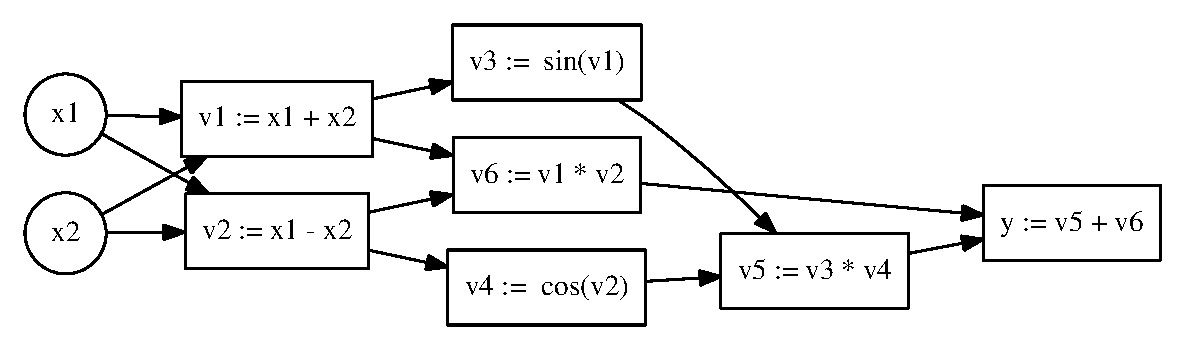
\epsfig{file=Figures/cg.eps,scale=0.8} \
\vspace*{-0.3cm}
\caption{Rendering of the computation graph shown in Figure \ref{fig:computational-graph}.}
\label{fig:cg.eps}
\end{figure}

\begin{Definition}[admissible]
A computational graph $G$ is \blue{admissible} \index{admissible, computational graph} if for every node of the form
\\[0.2cm]
\hspace*{1.3cm}
$\langle n, o, a_1, a_2\rangle$
\\[0.2cm]
that occurs in the list $G$ there are nodes labelled with $a_1$ and $a_2$ that occur in the list $G$ before this node and for
every  node of the form
\\[0.2cm]
\hspace*{1.3cm}
$\langle n, f, a\rangle$
\\[0.2cm]
that occurs in the list $G$ there is a node labelled with $a$ that occurs in the list G before this node.
If a computational graph is admissible, the nodes can be evaluated in the same order as they are listed in $G$.
\eoxs
\end{Definition}
\begin{figure}[!ht]
\centering
\begin{minted}[ frame         = lines, 
                 framesep      = 0.3cm, 
                 firstnumber   = 1,
                 bgcolor       = sepia,
                 numbers       = left,
                 numbersep     = -0.2cm,
                 xleftmargin   = 0.8cm,
                 xrightmargin  = 0.8cm,
               ]{python3}
    def eval_graph(CG, Values):
        for node in CG:
            match node:
                case (v, ):
                    pass
                case (v, r):
                    Values[v] = r
                case (v, '+', a1, a2):
                    Values[v] = Values[a1] + Values[a2]
                case (v, '-', a1, a2):
                    Values[v] = Values[a1] - Values[a2]
                case (v, '*', a1, a2):
                    Values[v] = Values[a1] * Values[a2]
                case (v, '/', a1, a2):
                    Values[v] = Values[a1] / Values[a2]
                case (v, 'sqrt', a):
                    Values[v] = math.sqrt(Values[a])            
                case (v, 'exp', a):
                    Values[v] = math.exp(Values[a])
                case (v, 'log', a):
                    Values[v] = math.log(Values[a])
                case (v, 'sin', a):
                    Values[v] = math.sin(Values[a])
                case (v, 'cos', a):
                    Values[v] = math.cos(Values[a])
                case (v, 'atan', a):
                    Values[v] = math.atan(Values[a])
        return Values['y']
\end{minted}
\vspace*{-0.3cm}
\caption{A function that evaluates a computational graph.}
\label{fig:Reverse-Mode-AD.ipynb:eval_graph}
\end{figure}

In order to \blue{evaluate} an admissible computational graph that contains $n$ variables, we will assume that the first
$n$ nodes are labelled with the variables $\mathtt{x}_1$, $\cdots$, $\mathtt{x}_n$ and that the last node in a computational node
is labelled with the name \texttt{y}.  Furthermore, we need a dictionary \texttt{Values} that assigns a value to each
of the variables $\mathtt{x}_1$, $\cdots$, $\mathtt{x}_n$.  Then the function \texttt{eval\_graph} that is shown in Figure
\ref{fig:Reverse-Mode-AD.ipynb:eval_graph} can be used to evaluate the nodes of the computational graph
\texttt{CG} one by one.  The idea is that initially the dictionary \texttt{Values} maps all variables to
floating point values.  Then the nodes of the computational graph are evaluated one by one.  For example, if a
node of the form
\\[0.2cm]
\hspace*{1.3cm}
$\langle v, \texttt{'+'}, a_1, a_2 \rangle$
\\[0.2cm]
has to be evaluated, then we can assume that the nodes that are labelled with $a_1$ and $a_2$ have already been
evaluated and that their values are stored in the dictionary \texttt{Values}.  These values are added and the
resulting value is stored under the key $v$ in the dictionary \texttt{Values}.

In the following we will assume that all computational graphs are admissible.
The crucial definition in the theory of reverse mode automatic differentiation is the notion of an
\blue{adjoint}, which will be given later after we have defined to notion of a \blue{parent} of a node.  
\FloatBarrier

\begin{figure}[!ht]
\centering
\begin{minted}[ frame         = lines, 
                 framesep      = 0.3cm, 
                 firstnumber   = 1,
                 bgcolor       = sepia,
                 numbers       = left,
                 numbersep     = -0.2cm,
                 xleftmargin   = 0.8cm,
                 xrightmargin  = 0.8cm,
               ]{python3}
    def parents(CG):
        Parents = {}
        for node in CG:
            match node:
                case (p, _, a):
                    add_to_dictionary(Parents, a, p)
                case (p, _, a1, a2):
                    add_to_dictionary(Parents, a1, p)
                    add_to_dictionary(Parents, a2, p)
        return Parents                 
    
    def add_to_dictionary(D, key, value):
        if key in D:
            D[key] |= { value }
        else:
            D[key]  = { value }
    
    def node_dictionary(CG):
        D = {}
        for node in CG:
            name    = node[0]
            D[name] = node
        return D
\end{minted}
\vspace*{-0.3cm}
\caption{Auxiliary functions.}
\label{fig:Reverse-Mode-AD.ipynb:auxiliary}
\end{figure}

\begin{Definition}[Parent]
  If $G$ is a computational graph and $\langle v, o, a_1, a_2\rangle$ is a node in $G$, then $v$ is a parent
  of the nodes that are labelled with $a_1$ and $a_2$.  Furthermore, if $\langle v, f, a\rangle$ is a node in
  $G$, then $v$ is a parent of the node that is labelled with $a$.
  \eoxs
\end{Definition}

Figure \ref{fig:Reverse-Mode-AD.ipynb:auxiliary} shows the implementation of the function \texttt{parents}
that can be used to compute the parents of a node.  It also contains the auxiliary function
\texttt{node\_dictionary} that takes a computational graph \texttt{CG} as its argument and returns a dictionary
associating every node with its name.
\FloatBarrier

\begin{Definition}[Adjoint]
  Assume $G$ is a computational graph such that the last node is labelled with then name \texttt{y}.
  If $v$ is any node in $G$, then the \blue{adjoint} \index{adjoint} of $v$, which is written as $\bar{v}$, is defined
  as the partial derivative of the output variable \texttt{y} w.r.t.~$v$, i.e.
  \\[0.2cm]
  \hspace*{1.3cm}
  $\ds\bar{v} := \frac{\partial \mathtt{y}}{\partial v}$.  \eoxs
\end{Definition}

\noindent
The next theorem is an immediate consequence of the 
\href{https://en.wikipedia.org/wiki/Chain_rule#Multivariable_case}{multivariable chain rule}.

\begin{Theorem}
  Assume $v$ is a node of a computational graph $G$ and that $p_1, \cdots, p_k$ are all the parents of this node
  in $G$. Then the adjoint $\bar{v}$ of the node $v$
  is given as
  \\[0.2cm]
  \hspace*{1.3cm}
  $\ds\bar{v} = \frac{\partial y}{\partial v} 
              = \sum\limits_{i=1}^k \frac{\partial y}{\partial p_i} \cdot \frac{\partial p_i}{\partial v}
              = \sum\limits_{i=1}^k \bar{p}_i \cdot \frac{\partial p_i}{\partial v}
  $.
\end{Theorem}

\example
To keep things simple, assume that the variables $\mathtt{x}_1$ and $\mathtt{x}_2$ that are shown in the
computational graph in Figure \ref{fig:cg.eps} are both initialized with the value $\pi/4$.
Before the adjoints can be computed, we have to compute the values associated with the nodes.
These are as follows:
\begin{enumerate}
\item $\mathtt{v}_1 = \pi/2$,
\item $\mathtt{v}_2 = 0$,
\item $\mathtt{v}_3 = 1$,
\item $\mathtt{v}_4 = 1$,
\item $\mathtt{v}_5 = 1$,
\item $\mathtt{v}_6 = 0$,
\item $\mathtt{y} = 1$.
\end{enumerate}
Next, we compute the adjoints.
\begin{enumerate}
\item $\ds \bar{\mathtt{y}} = \frac{\partial \mathtt{y}}{\partial \mathtt{y}} = 1$,
\item $\ds \bar{\mathtt{v}}_6 = \frac{\partial \mathtt{y}}{\partial \mathtt{v}_6} = 1$,
\item $\ds \bar{\mathtt{v}}_5 = \frac{\partial \mathtt{y}}{\partial \mathtt{v}_5} = 1$.
\item $\ds \bar{\mathtt{v}}_4 =
       \frac{\partial \mathtt{y}}{\partial \mathtt{v}_5} \cdot  \frac{\partial \mathtt{v}_5}{\partial \mathtt{v}_4}
       = \bar{\mathtt{v}}_5 \cdot \mathtt{v}_3 = 1 \cdot 1 = 1$.
\item $\ds \bar{\mathtt{v}}_3 =
       \frac{\partial \mathtt{y}}{\partial \mathtt{v}_5} \cdot  \frac{\partial \mathtt{v}_5}{\partial \mathtt{v}_3}
       = \bar{\mathtt{v}}_5 \cdot \mathtt{v}_4 = 1 \cdot 1 = 1$.
\item $\ds \bar{\mathtt{v}}_2 =
       \frac{\partial \mathtt{y}}{\partial \mathtt{v}_6} \cdot  \frac{\partial \mathtt{v}_6}{\partial \mathtt{v}_2} +
       \frac{\partial \mathtt{y}}{\partial \mathtt{v}_4} \cdot  \frac{\partial \mathtt{v}_4}{\partial \mathtt{v}_2} 
       = \bar{\mathtt{v}}_6 \cdot \mathtt{v}_1 - \bar{\mathtt{v}}_4 \cdot \sin(\mathtt{v}_2)
          = 1 \cdot \pi/2 - 1 \cdot \sin(0) = \pi/2 - 1 \cdot 0 = \pi/2$.
\item $\ds \bar{\mathtt{v}}_1 =
       \frac{\partial \mathtt{y}}{\partial \mathtt{v}_6} \cdot  \frac{\partial \mathtt{v}_6}{\partial \mathtt{v}_1} +
       \frac{\partial \mathtt{y}}{\partial \mathtt{v}_3} \cdot  \frac{\partial \mathtt{v}_3}{\partial \mathtt{v}_1} 
       = \bar{\mathtt{v}}_6 \cdot \mathtt{v}_2 + \bar{\mathtt{v}}_3 \cdot \cos(\mathtt{v}_1)
          = 1 \cdot 0 + 1 \cdot \cos(\pi/2) = 0 + 0 = 0$.
\item $\ds \bar{\mathtt{x}}_1 =
       \frac{\partial \mathtt{y}}{\partial \mathtt{v}_1} \cdot  \frac{\partial \mathtt{v}_1}{\partial \mathtt{x}_1} +
       \frac{\partial \mathtt{y}}{\partial \mathtt{v}_2} \cdot  \frac{\partial \mathtt{v}_2}{\partial \mathtt{x}_1} 
       = \bar{\mathtt{v}}_1 \cdot 1 + \bar{\mathtt{v}}_2 \cdot 1
          = 0 \cdot 1 + \pi/2 \cdot 1 = \pi/2$.
\item $\ds \bar{\mathtt{x}}_2 =
       \frac{\partial \mathtt{y}}{\partial \mathtt{v}_1} \cdot  \frac{\partial \mathtt{v}_1}{\partial \mathtt{x}_2} +
       \frac{\partial \mathtt{y}}{\partial \mathtt{v}_2} \cdot  \frac{\partial \mathtt{v}_2}{\partial \mathtt{x}_2} 
       = \bar{\mathtt{v}}_1 \cdot 1 + \bar{\mathtt{v}}_2 \cdot (-1)
       = 0 \cdot 1 + \pi/2 \cdot (-1) = - \pi/2$.
\end{enumerate}
Hence we have shown the following:
\\[0.2cm]
\hspace*{1.3cm}
$\ds \frac{\partial \mathtt{y}}{\partial \mathtt{x}_1}\Bigl(\frac{\pi}{4}, \frac{\pi}{4}\Bigr) = \frac{\pi}{2}$ \quad and \quad
$\ds \frac{\partial \mathtt{y}}{\partial \mathtt{x}_2}\Bigl(\frac{\pi}{4}, \frac{\pi}{4}\Bigr) = - \frac{\pi}{2}$.
\\[0.2cm]     
Note that we have found the exact partial derivatives for a specific point, namely for the arguments
$\mathtt{x}_1 = \pi/4$ and $\mathtt{x}_2 = \pi/4$.  Automatic differentiation is not symbolic differentiation
and hence is not able to derive general formulas but rather computes values for specific arguments.  However,
these values are not numerical approximations but are, instead, exact.
\eoxs

\begin{figure}[!ht]
\centering
\begin{minted}[ frame         = lines, 
                 framesep      = 0.3cm, 
                 firstnumber   = 1,
                 bgcolor       = sepia,
                 numbers       = left,
                 numbersep     = -0.2cm,
                 xleftmargin   = 0.8cm,
                 xrightmargin  = 0.8cm,
               ]{python3}
    def partial_derivative(Node, arg, Values):
        match Node:
            case n, '+', a1, a2:
                if arg == a1 == a2:
                    return 2
                if arg == a1 or arg == a2:
                    return 1
            case n, '-', a1, a2:
                if arg == a1 == a2:
                    return 0
                if arg == a1:
                    return 1
                if arg == a2:
                    return -1
            case n, '*', a1, a2:
                if arg == a1 == a2:
                    return 2 * Values[a1]
                if arg == a1:
                    return Values[a2]
                if arg == a2:
                    return Values[a1]
            case n, '/', a1, a2:
                if arg == a1 == a2:
                    return 0
                if arg == a1:
                    return 1 / Values[a2]
                if arg == a2:
                    return -Values[a1] / Values[a2] ** 2
            case n, 'sqrt', a:
                return 0.5 / math.sqrt(Values[a])
            case n, 'exp', a:
                return math.exp(Values[a])
            case n, 'log', a:
                return math.log(Values[a])
            case n, 'sin', a:
                return math.cos(Values[a])
            case n, 'cos', a:
                return -math.sin(Values[a])
            case n, 'atan', a:
                return 1 / (1 + Values[a]**2)
\end{minted}
\vspace*{-0.3cm}
\caption{Computing the partial derivative of a node.}
\label{fig:Reverse-Mode-AD.ipynb:partial_derivative}
\end{figure}

Of course, we do not want to perform computations like the following ourselves.  The function
\texttt{partial\_derivative} shown in Figure \ref{fig:Reverse-Mode-AD.ipynb:partial_derivative} takes a
computational \texttt{Node} and computes the partial derivative of this node with respect to the given
argument \texttt{arg}.  The last argument \texttt{Values} is a dictionary containing the values that are
associated with the different nodes.
\FloatBarrier


\begin{figure}[h]
\centering
\begin{minted}[ frame         = lines, 
                 framesep      = 0.3cm, 
                 firstnumber   = 1,
                 bgcolor       = sepia,
                 numbers       = left,
                 numbersep     = -0.2cm,
                 xleftmargin   = 0.8cm,
                 xrightmargin  = 0.8cm,
               ]{python3}
    def adjoints(CG, Values):
        eval_graph(CG, Values)
        NodeDict = node_dictionary(CG)
        Parents  = parents(CG)
        n        = len(CG)
        Adjoints = {}
        Adjoints['y'] = 1
        for k in range(2, n+1):
            Node   = CG[-k]
            name   = Node[0]
            result = 0
            for parent_name in Parents[name]:
                parent_node = NodeDict[parent_name]
                pd          = partial_derivative(parent_node, name, Values)
                result += Adjoints[parent_name] * pd
            Adjoints[name] = result
        return Adjoints
\end{minted}
\vspace*{-0.3cm}
\caption{Computing the adjoints of a computational graph.}
\label{fig:Reverse-Mode-AD.ipynb:adjoints}
\end{figure}


The function \texttt{adjoints} shown in Figure \ref{fig:Reverse-Mode-AD.ipynb:adjoints} computes the adjoints
of a given computational graph.  It needs a dictionary \texttt{Values} that maps the variables $x_1$, $\cdots$,
$x_n$ to their values.  It returns a dictionary that associates all node names with their adjoints.
\FloatBarrier





%%% Local Variables:
%%% mode: latex
%%% TeX-master: "artificial-intelligence"
%%% End:
